\documentclass[conference]{IEEEtran}
\IEEEoverridecommandlockouts
% The preceding line is only needed to identify funding in the first footnote. If that is unneeded, please comment it out.

\usepackage{amsmath,amssymb,amsfonts}
\usepackage{algorithmic}
\usepackage{graphicx}
\usepackage{textcomp}
\usepackage{xcolor}
\usepackage{enumitem}
\usepackage{float}


\def\BibTeX{{\rm B\kern-.05em{\sc i\kern-.025em b}\kern-.08em
    T\kern-.1667em\lower.7ex\hbox{E}\kern-.125emX}}
\setlist[itemize]{label=$\bullet$}

\begin{document}

\title{Comparing Model-View-Controller (MVC) VS Model-View-Presenter (MVP) In Terms of Speed and Memory Usage \\
}
\author{\IEEEauthorblockN{1\textsuperscript{st} Alexander Dennis Ong}
\IEEEauthorblockA{\textit{Pradita University} \\
\textit{Information Technology 2022}\\
Tangerang, Indonesia \\
alexander.dennis@student.pradita.ac.id}
\and
\IEEEauthorblockN{2\textsuperscript{nd} Arnold Christopher Ghazali}
\IEEEauthorblockA{\textit{Pradita University} \\
\textit{Information Technology 2022}\\
Tangerang, Indonesia \\
arnold.christopher@student.pradita.ac.id}
\and
\IEEEauthorblockN{3\textsuperscript{rd} Okhama Siladata Devisepte}
\IEEEauthorblockA{\textit{Pradita University} \\
\textit{Information Technology 2022}\\
Tangerang, Indonesia \\
okhama.siladata@student.pradita.ac.id}
\and
\IEEEauthorblockN{4\textsuperscript{th} Brandon Josua Christian}
\IEEEauthorblockA{\textit{Pradita University} \\
\textit{Information Technology 2022}\\
Tangerang, Indonesia \\
brandon.josua@student.pradita.ac.id}

}

\maketitle

\begin{abstract}
The choice of architectural patterns significantly influences the performance and memory efficiency of software systems. In this paper, we present a comprehensive comparative analysis between two widely used architectural patterns: Model-View-Controller (MVC) and Model-View-Presenter (MVP). Our study aims to provide insights into which architectural pattern is superior concerning speed and memory usage, crucial factors in determining the scalability and responsiveness of modern applications.

To conduct a fair evaluation, we implemented identical applications using both MVC and MVP architectures. We developed benchmarks to measure the speed of execution and memory footprint of each pattern under various scenarios, including different input sizes and complexities. 

Furthermore, we discuss the implications of these findings on software development practices and provide recommendations for selecting the most suitable architectural pattern based on specific project requirements. By offering empirical evidence and insights into the performance attributes of MVC and MVP, this study contributes to informed decision-making in architectural design, ultimately enhancing the overall quality and efficiency of software systems. 

(*BELOM SELESAI*)
\end{abstract}

\section{Introduction}
Software development has undergone a significantly significant evolution in recent decades, with the emergence of various design patterns to build more structured and maintainable applications. 

In software development, Model View Controller (MVC) and Model View Presenter (MVP) are two frequently debated design patterns. MVC, which emerged in the 1970s, organizes applications into Model (data), View (presentation), and Controller (logic) components. On the other hand, MVP is a variation of MVC that emerged in the early 2000s, introducing the Presenter as an intermediary between the Model and View to separate presentation logic from business logic. Comparing these two patterns is crucial for a better understanding of their strengths, weaknesses, and suitable applications in software development.

This research aims to delve into the comparison between the Model View Controller (MVC) and Model View Presenter (MVP) design patterns in software development. Through in-depth analysis of these two design patterns, it is hoped that the strengths, weaknesses, and optimal use cases for each pattern can be identified. Consequently, this study aims to provide valuable guidance for software developers in selecting the design pattern that best suits the needs of their projects.

\section{Related Studies}
\section*{The MVC Model}
\subsection{Understanding The MVC Architecture Model}

Utilizing graphical user interface (GUI) libraries simplifies the implementation of the model-view-controller (MVC) design pattern. Initially proposed by Trygve Reenskaug, a Smalltalk developer at Xerox Palo Alto Research Center in 1979, MVC facilitates the separation of data access and business logic from the presentation to the user [Fig 1]. To elaborate, the following figure is the representation of how to MVC Works \cite{dey2011comparative}.

\begin{figure}
    \centering
    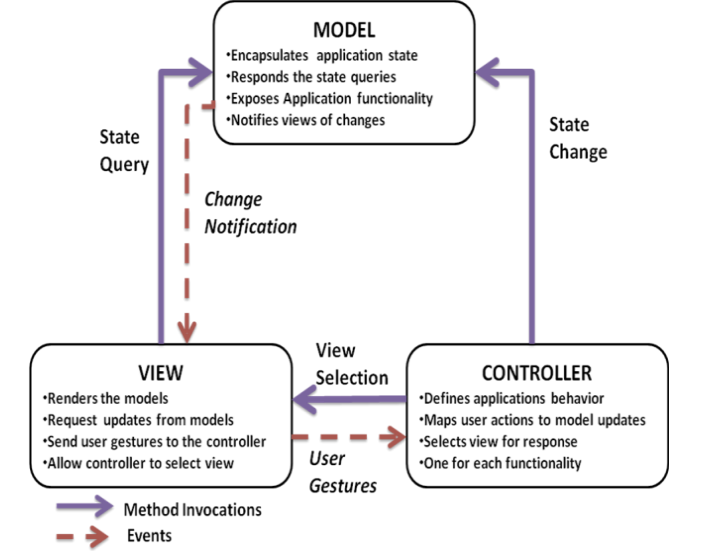
\includegraphics[width = 0.4\textwidth]{Image/Figure 1.PNG}
    \caption{MVC Model \cite{dey2011comparative}}
    \label{fig:enter-label}
\end{figure}

The Model Role is to act as an object that represent a data or a process of a program for example as a database and a process for the machines to act, application logic belong to this section \cite{thakur2019role}.
a model functions as a digital representation of real-world processes, embodying both the data and the regulations dictating its access and modification \cite{dey2011comparative}.

The View is a form of presentation of what the user will see when it request something, a user interface belong to this category \cite{thakur2019role}.

The view displays the information contained within a model and dictates the precise manner in which this data should be shown. When there are alterations to the model data, the view adjusts its presentation accordingly. This adjustment can be accomplished through either a push model, where the view subscribes to the model for updates, or a pull model, where the view actively requests the latest data from the model \cite{dey2011comparative}.

The controller interprets the user's interactions with the view and translates them into operations that the model will execute. In a standalone graphical user interface (GUI) client, these interactions might include clicking buttons or selecting menu options, while in an enterprise web application, they typically manifest as GET and POST HTTP requests. Depending on the situation, the controller might also determine which view to present to the user next, such as a page displaying search results in a web application \cite{dey2011comparative}.

\subsection{An example of how the MVC Works}

This is an example of a web browser about a movie. The user in this example want to see list of movies available on the web and this is how the MVC works[fig 2].

\begin{figure}
    [h]
    \centering
    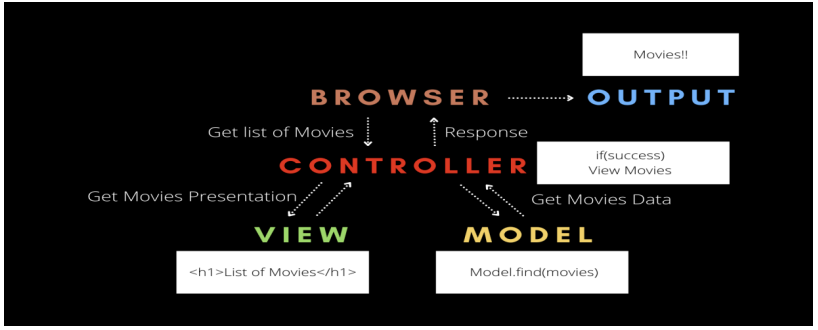
\includegraphics[width = 0.4\textwidth]{Image/figure 2.PNG}
    \caption{MVC flow example \cite{rustagi2022mvc}}
    \label{fig:enter-label}
\end{figure}

So in this case the user input the data about a list of movies this is what happens. 
In the process of retrieving a list of movies, the browser initiates a request to the Controller, which subsequently communicates with the Model to fetch the desired data from the primary database. Once the Model retrieves the list of movies, it delivers it to the Controller. If the Controller successfully obtains the list, it directs the View to render the movies in HTML format. The View then generates the HTML representation of the movie list, which is returned to the Controller. Finally, the Controller presents this HTML to the user, resulting in the display of the list of movies \cite{rustagi2022mvc}.

\subsection{MVC utilization}
\begin{itemize}
\item MVC or model view controller is highlighted for its ability to streamline horizontal development and maintenance of large scale distributed web application across three frameworks: Big Blob, MVC architecture, and modified MVC Design.
\item The Model-View-Controller (MVC) architecture is easier to implement graphical user interface (GUI) libraries because it provides a true decoupling of each part. So it is easier to change the odel part and view will notify the update the model does not carry a refenrence to the view but instead uses an event-notification model to notify interested parties of a change. One of the problem using this powerful design is that the many views can have the same underlying model. When a change in the data model occurs, each view is notified by a property change event and can update itself accordingly.
\item The Modifying MVC architecture uses Cocoa Touch
frameworks that power Mac OS X and iOS are tightly integrated
into the Xcode development experience. Cocoa’s high-level
APIs make it easy to add animation, networking, and the native
platform appearance and behavior to your application with only
a few lines of code. In this Structure models encapsulate
application data, Views display and edit that data, and
Controllers mediate the logic between the two. By separating
responsibilities in this manner, you end up with an application
that is easier to design, implement, and maintain
\item The MVC architecture was able to solve some of the problem of
web and internet programming but still there were a lot of things
missing from it. It was centred on the navigation of the JSP
pages so there was the scope of the further development in the
architecture point of view. During this process the next
development was the Model 2 architecture. This problem was
solved using the Servlet and JSP together. The Servlet handles
the Initial request and partially process the data. It set up the
beans then forward the result to the one of the JSP page. The
Servlet decide the one of the page to be displayed from the list of
pages


\subsection{Advantages and Disadvantages of MVC}
\begin{enumerate}
    \item Advantages of MVC
\begin{itemize}
    \item Separation of Concerns: MVC enforces a clear separation between the data (Model), the presentation logic (View), and the application logic (Controller). This separation makes the codebase easier to understand, maintain, and extend.
    \item Modularity: Each component in MVC can be developed independently of the others. This modularity allows developers to work on different parts of the application simultaneously without interfering with each other's work.
    \item Reusability: Components in MVC can often be reused across different parts of the application or even in entirely different applications. For example, a controller logic that handles user authentication can be reused in multiple views.
    \item Testability: Because of its separation of concerns, each component in MVC can be unit tested independently, which makes it easier to write automated tests for the application.
    \item Scalability: MVC promotes a structure that scales well with the size and complexity of the application. As the application grows, developers can add more models, views, and controllers without significantly impacting existing code.
\end{itemize}
\item Disadvantages of MVC
\begin{itemize}
\item Complexity: Implementing MVC requires a good understanding of the pattern and its principles. For developers unfamiliar with MVC, there may be a learning curve associated with adopting this architectural pattern.
\item Overhead: MVC can introduce some additional overhead compared to simpler architectures, particularly in terms of initial setup and configuration. In some cases, MVC might be overkill for small or simple applications.
\item Tight Coupling: While MVC aims to reduce dependencies between components, it's still possible to introduce tight coupling between the components, especially if not implemented properly. Tight coupling can make the code harder to maintain and refactor.
\item Potential for Code Duplication: Without proper discipline, developers might duplicate code across different components of the MVC architecture, leading to maintenance issues and inconsistencies.
\item Increased Complexity in Asynchronous Applications: Asynchronous programming and handling asynchronous requests in MVC can sometimes introduce additional complexity, especially in scenarios where the flow of control is not linear.
\end{itemize}
\end{enumerate}
\end{itemize}
\section*{The MVP Model}
\subsection{Understanding The MVP Architecture Model}

The MVP is designed around two questions: data management and user interface. It's about how data is managed and how  users interact with the data. There are six components that recognized in MVP architecture: model, selections, commands, presenter, interactor and view. The model component is like the concept in MVC that indicates what  data is present in this application. The Selection element specifies the subset  of the data to be used. The Command component presents a list of actions that can  be performed. The View component is the same in MVC. The Interactor component indicates which events should be triggered by the user, e.g. keyboard, mouse movements and clicks, scrolling. The Presenter component is like a controller in MVC that is intended to organize and coordinate all the intermediary components – interactors, options, and commands. The first three components are for data management and the last three part is for the user interface.

Most of the time MVP architecture is described as consisting 3 components: model, view and presenter. Interactors, controls, and selections are placed in the presenter component.
With MVP, the coupling between view and model is eliminated. The model knows nothing about the presenter and vice versa \cite{c5}.
MVP model interaction are desribed in Figure 3.

\begin{figure}
    [h]
`   \centering
    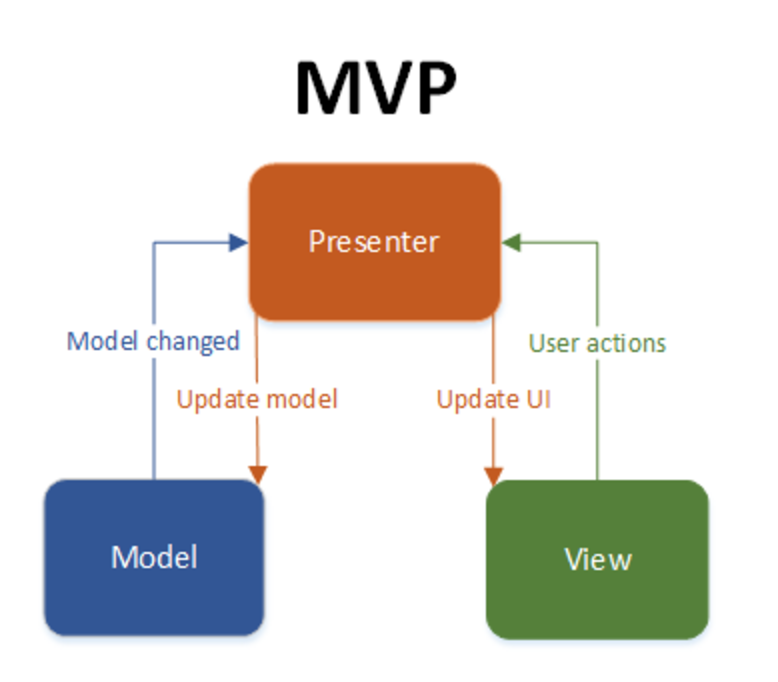
\includegraphics[width = 0.4\textwidth]{Image/MVP model.png}
    \caption{MVP Model}
\end{figure}

The flow of MVP starts from view component. View capture user actions and send them to presenter. For a simple action, presenter makes decision and update the view. If this a complex action, the presenter will send message to the model to get the relevant data and then update the view. Sometimes user action impacts model data. In this case the View will not directly affect the model but requires the presenter to update the model \cite{c5}. 

\subsection{Advantages and Disadvantages of MVP}
\begin{enumerate}
    \item Advantages of MVP
\begin{itemize}
    \item MVP aims to reinforce the separation between the main components of the application: the model, view, and presenter. With clear separation, developers can more easily manage and maintain code as each component has well-defined responsibilities. This helps avoid complex code stacks and facilitates additional development or changes in the future \cite{Lappalainen2017APL}.
    \item The MVP is its ability to support automated testing of the user interface. By separating presentation logic from the view, unit testing can focus on the presenter without directly involving the view. This facilitates the testing process and allows developers to effectively validate application behavior automatically \cite{Lappalainen2017APL}.
    \item MVP variations, especially in the form of Passive View, offer significant testing convenience. By separating presentation logic from the view, unit testing can be done in isolation for the presenter and model. This reduces dependency on the view and enables more focused and efficient testing, helping to identify and fix bugs more quickly \cite{Lappalainen2017APL}.
    \item Both Supervising Controller and Passive View patterns in MVP have a significant testing footprint. This means that applications built using these patterns have broader testing capabilities, allowing developers to conduct comprehensive testing and better maintain applications \cite{Lappalainen2017APL}.
    \item MVP is a design pattern that separates the presenter, view, and model in an application, providing greater flexibility in dividing responsibilities within it. Each component has well-defined roles, allowing developers to efficiently manage the application logic and modify or extend functionality without disrupting other components. This helps strengthen the application architecture and makes it easier to organize and maintain over time \cite{Lappalainen2017APL}.
\end{itemize}
\item Disadvantages of MVP
\begin{itemize}
\item The drawback of MVP is the potential for low re-usability because the presenter is tasked with updating the view. This could result in code that is challenging to reuse across various sections of the application \cite{Lappalainen2017APL}.
\item A disadvantage of MVP is the likelihood of low separation of concerns, particularly in the Passive View pattern, where the presenter is responsible for view updates. This may lead to increased code complexity and impede application maintenance \cite{Lappalainen2017APL}.
\item An issue with MVP is the difficulty in maintaining the application, especially in the Passive View pattern, due to potential code complexity. This challenge arises primarily when the presenter is responsible for updating the view \cite{Lappalainen2017APL}.
\end{itemize}
\end{enumerate}

\subsection{Difference Between MVC and MVP Architecture}
In MVP (Model-View-Presenter), the view directly communicates with the presenter, making it easy to supply user information for a specific model. The role of the view is strictly for displaying data and does not implement any business logic. Multiple views can be associated with the same presenter, allowing for flexibility in the user interface \cite{c2}.

In contrast, MVC (Model-View-Controller) allows for multiple controllers to handle views, especially in web applications where different events like mouse clicks or keyboard inputs may trigger actions. The controller manages the interaction between the model and the view \cite{c2}.

The presenter in MVP acts as an intermediary between the view and the model, reading and retrieving data from the model through the view interface. This separation ensures that business logic remains within the presenter and model layers \cite{c2}.

The model's role is consistent across both MVP and MVC, containing the business data and functionality associated with it. However, in MVP, the model does not have a direct reference to the presenter, leading to the need for page refreshes to update data, unlike MVC where updates can occur without refreshing the page \cite{c2}.

\subsection{Planning and Implementation}
As a architechture both the MVC and the MVP although a bit similar the difference between the structure is as follow, 

In the MVC framework, both the view and the controller are part of the user interface. Initially, a user makes a request to a controller via a graphical user interface (GUI). The controller then interacts with the model to retrieve the relevant data based on the user’s request. Once the model returns the data, the controller processes it and displays the information through the designated view \cite{c6}.

\begin{figure}
    [h]
    \centering
    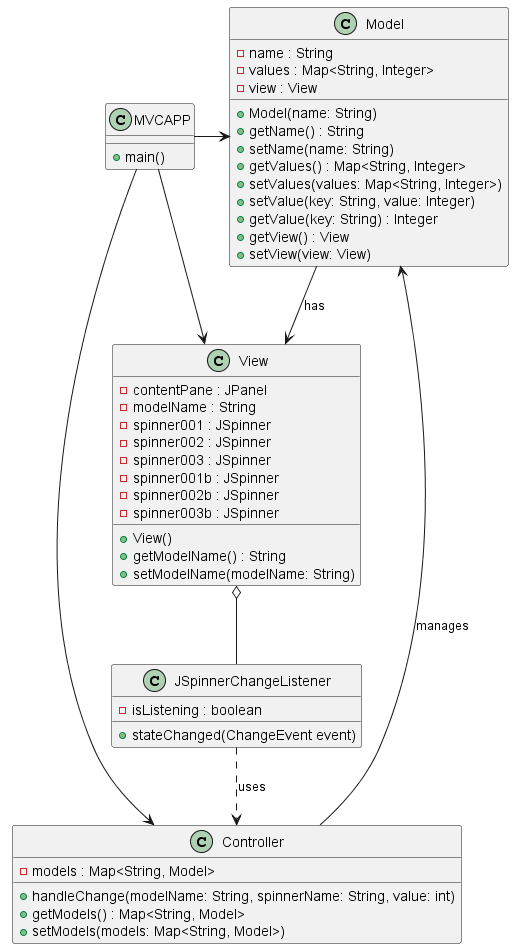
\includegraphics[width = 0.4\textwidth]{Image/mvc_class_diagram.png}
    \caption{MVC class diagram}
    \label{fig:enter-label}
\end{figure}

\begin{figure}
    [h]
    \centering
    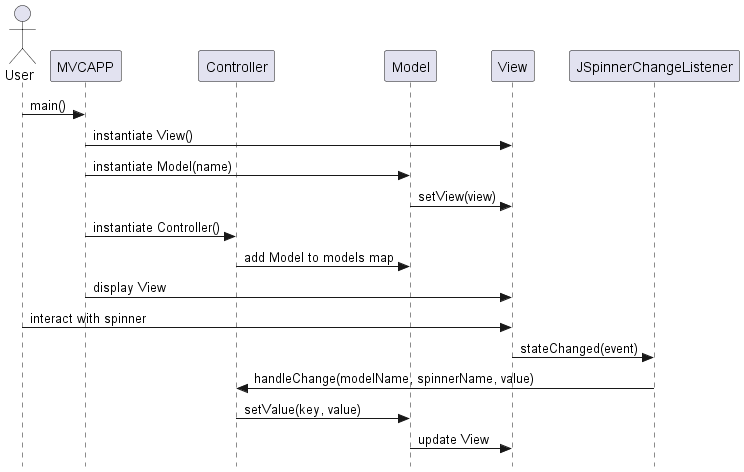
\includegraphics[width = 0.4\textwidth]{Image/mvc_sequence_diagram.png}
    \caption{MVC sequence diagram}
    \label{fig:enter-label}
\end{figure}

The sequence diagram (Figure 5) illustrates the interaction flow within an MVC application, detailing how the user interacts with the system and how different components communicate. Initially, the user triggers the main() method in the MVCAPP, which leads to the instantiation of the View. Subsequently, a Model is instantiated with a specific name and the View is set within the Model. A Controller is then instantiated, and the Model is added to a models map managed by the Controller. The View is then displayed to the user.

As the user interacts with a spinner component within the View, a JSpinnerChangeListener detects this change, invoking the stateChanged(event) method. This event triggers the handleChange(modelName, spinnerName, value) method in the Controller, which updates the Model by calling the setValue(key, value) method. The Model then communicates back to the View to update its display accordingly, reflecting the new state resulting from the user's interaction. This sequence ensures a clear separation of concerns, with each component handling its specific responsibilities in the MVC architecture.

the MVP Architecture on the other hand differs from the MVC Architecture by shifting the responsibility for data retrieval and business logic to the Presenter. The Presenter interacts with the Model to get data, processes the business logic, and then updates the View with the results. In MVP Architecture, UI-related logic such as data selection and classification, which is handled by the View in MVC, is managed by the Presenter instead. This design ensures that the View is only responsible for displaying the UI, maintaining a not so tight relation with its corresponding Presenter \cite{c7}.

\begin{figure}
    [h]
    \centering
    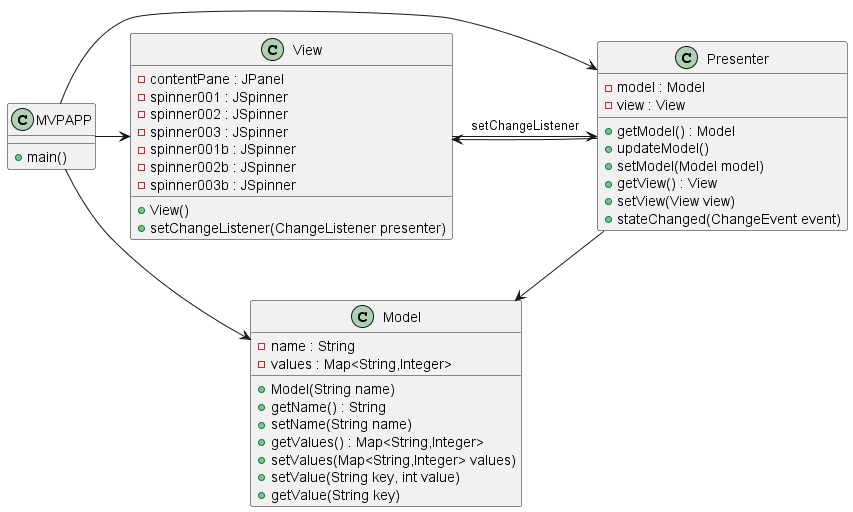
\includegraphics[width = 0.5\textwidth]{Image/mvp_class_diagram.png}
    \caption{MVP class diagram}
    \label{fig:enter-label}
\end{figure}

\begin{figure}
    [h]
    \centering
    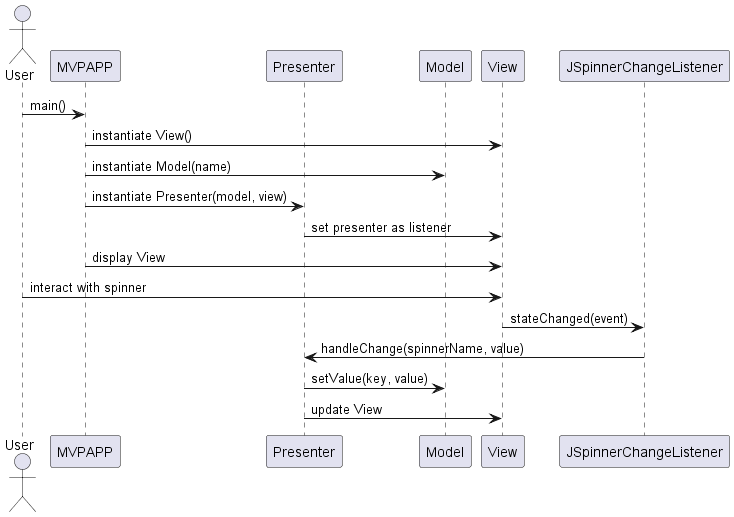
\includegraphics[width = 0.4\textwidth]{Image/mvp_sequence_diagram.png}
    \caption{MVP sequence diagram}
    \label{fig:enter-label}
\end{figure}
The sequence diagram (Figure 7) illustrates the workflow within an MVP (Model-View-Presenter) application. Initially, the user triggers the main() method in the MVPAPP, which leads to the instantiation of the View and the Model with a specified name. Following this, a Presenter is instantiated, taking both the Model and the View as parameters, and sets itself as a listener for the View. The View is then displayed to the user.

When the user interacts with a spinner component within the View, a JSpinnerChangeListener detects this change and triggers the stateChanged(event) method. This event calls the handleChange(spinnerName, value) method in the Presenter, which updates the Model by invoking the setValue(key, value) method. Once the Model is updated, the Presenter instructs the View to refresh its display through the update View method. This interaction sequence demonstrates how the MVP pattern delegates the business logic to the Presenter, while the View remains focused solely on the UI presentation.
\section{Methodology}
in this experiment to determine which software architechture performs better is using the following method. Each experiment consists of 10 instances of MV*. In the first instance, the view contains only 1 JSpinner. In the second instance, the view contains 2 JSpinner. In the 100th instance, the view contains 100 JSpinner. Change the value of all JSpinner from View 1 to View 100. Record the time taken to complete the operation. Repeat the experiment 15 times. And using python matplotlib to produce the graphs necessary for the research.
The experiments were conducted on a desktop with a 4 core processor and 16 GB of RAM.
\section{results and discussion}
\subsection{MVC Test Results}
The MVC architechture finished the experiment with 5.7 minutes with the following data produced that representated using matplotlib as following


\begin{figure}
    [h]
    \centering
    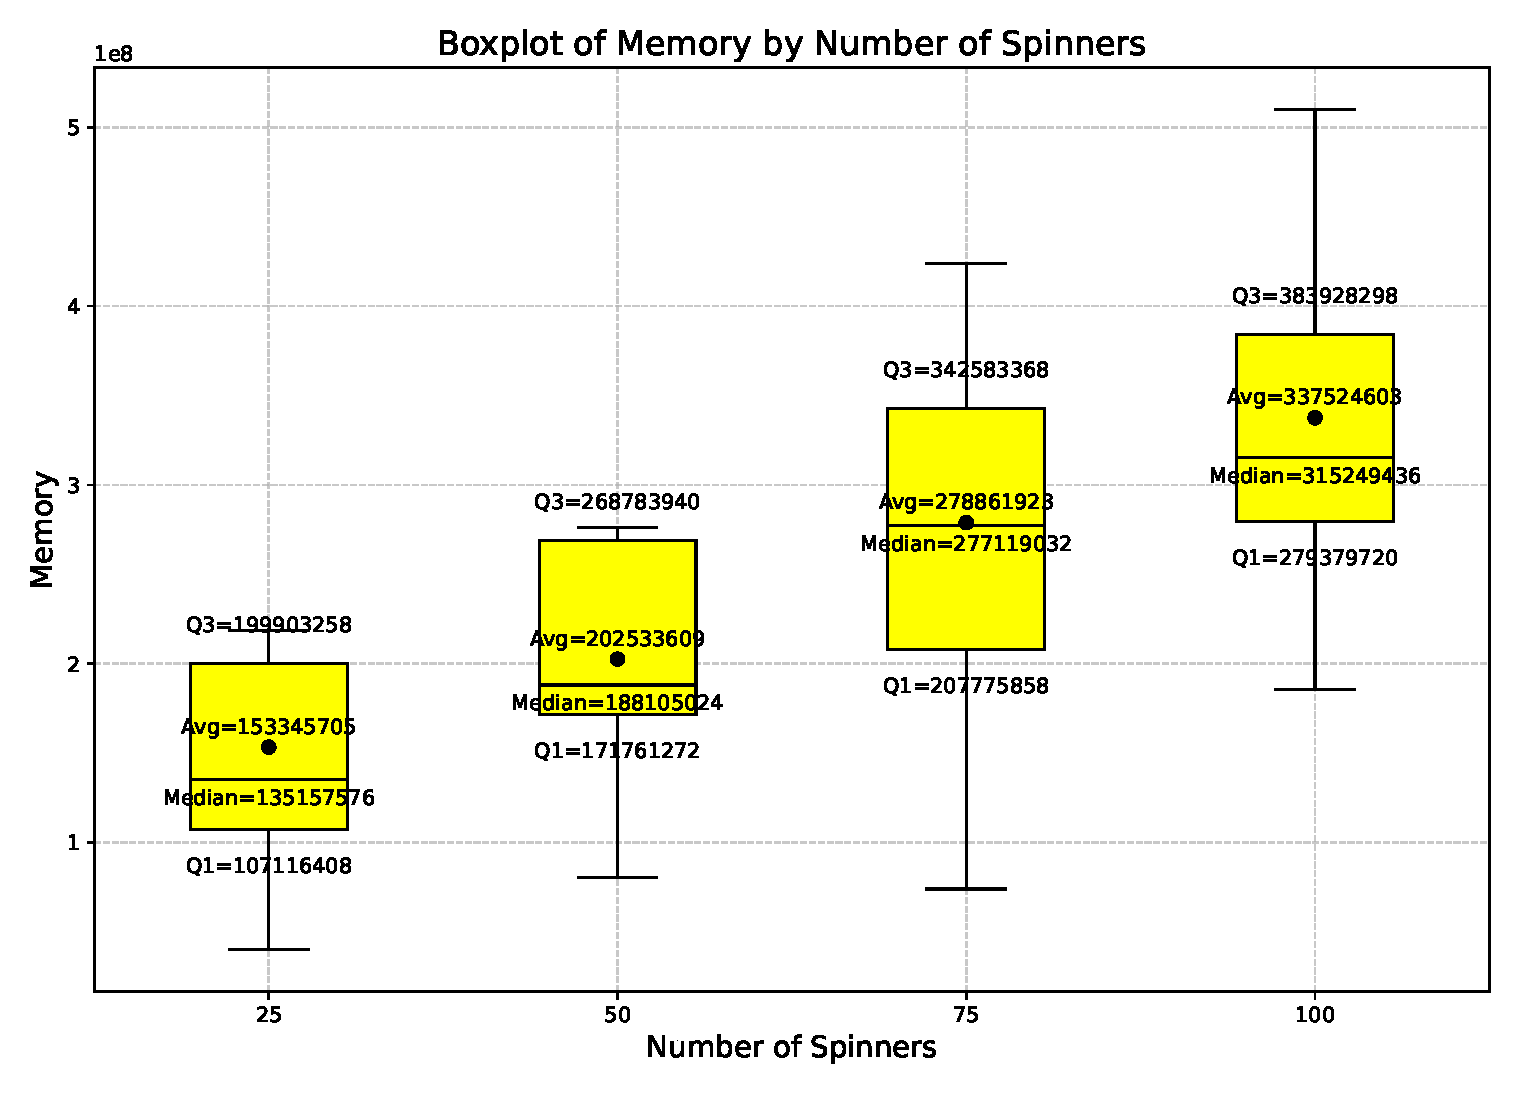
\includegraphics[width = 0.3\textwidth]{Image/mvc_plot_spin_total_memory.pdf}
    \caption{Memory Used With The Number Of Spinners Used (mvc)}
    \label{fig:enter-label}
\end{figure}

from the plot on figure 8, it indicates a clear increase that the more spinners used will also increase the memory usage when testing the program. But from figure 9, we can see that the number of spinners doesn't affect the time it needs to complete the task
\begin{figure}
    [h]
    \centering
    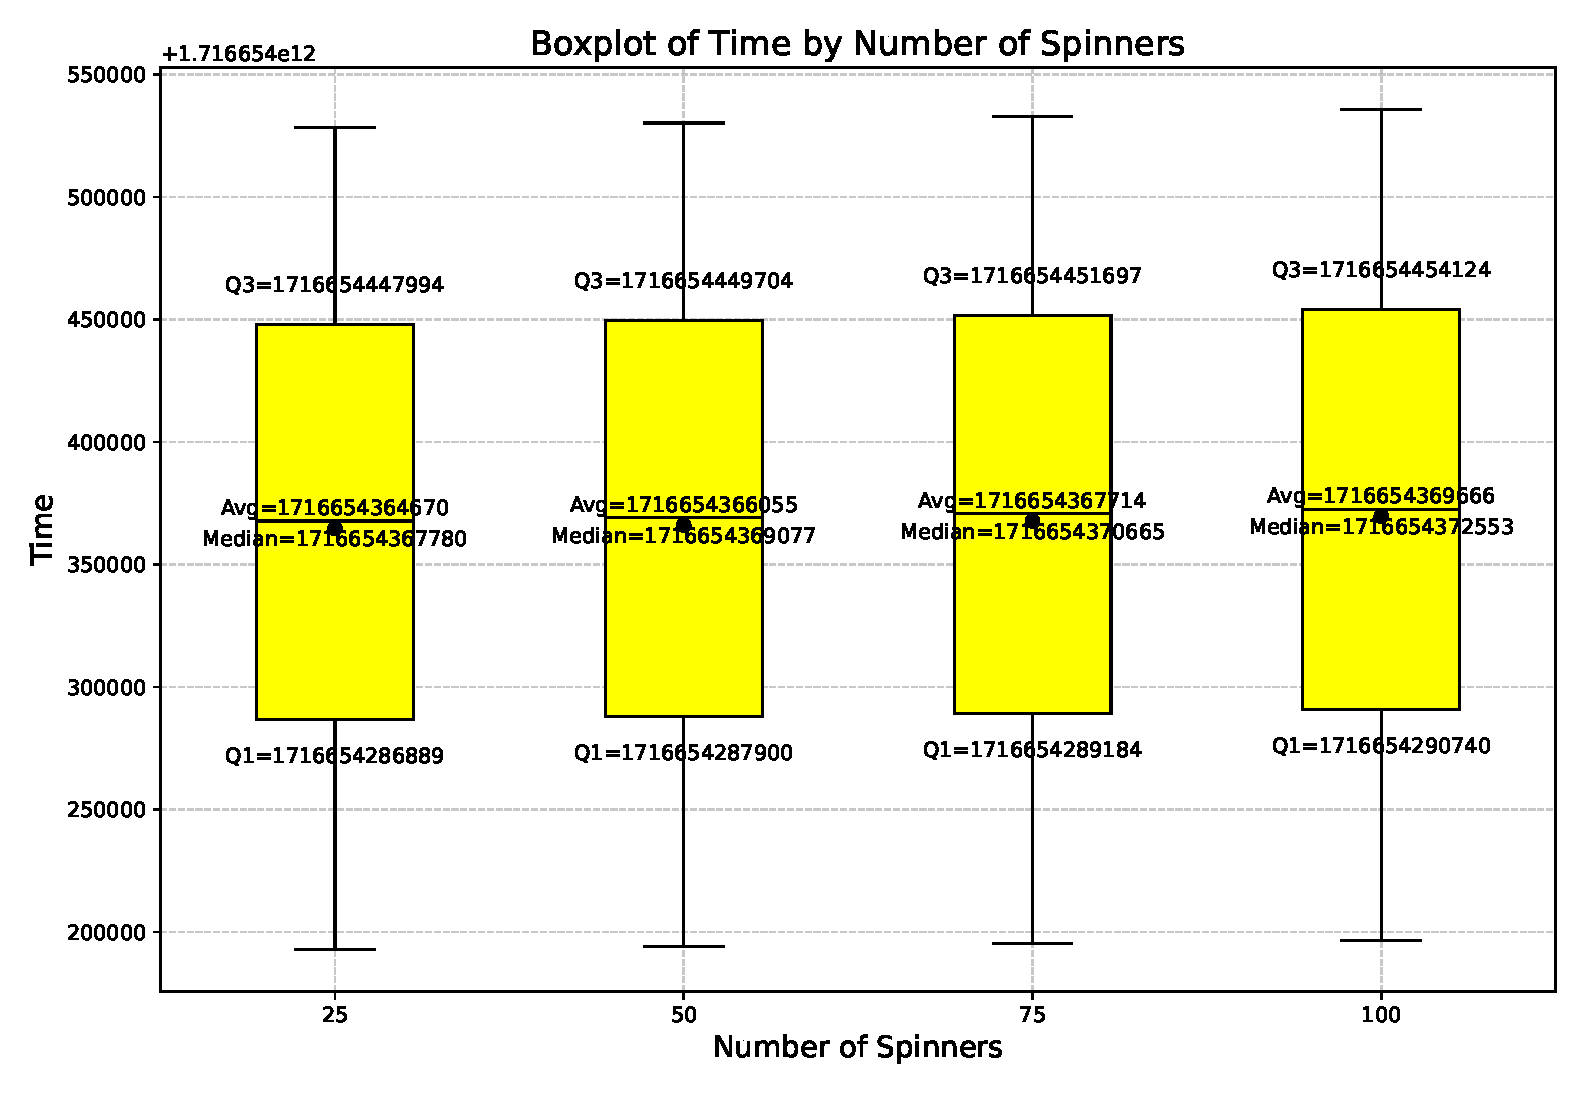
\includegraphics[width = 0.3\textwidth]{Image/mvc_plot_spin_total_time.pdf}
    \caption{Times needed With The Number Of Spinners Used (mvc)}
    \label{fig:enter-label}
\end{figure}

From Figure 10,it indicates a clear increase in memory usage as the number of views increases. This suggests that as more views are added, the program requires more memory to handle the additional data and interactions. Furthermore, the time needed to complete the task also increases, although this increase is relatively slight. As shown in Figure 11, the time required to complete the task grows marginally longer with the addition of more views. This indicates that while memory usage scales significantly with the number of views, the impact on the overall completion time is less pronounced but still noticeable. Together, these observations highlight the trade-offs between memory consumption and processing time in the program as the complexity and number of views increase.

\begin{figure}
    [h]
    \centering
    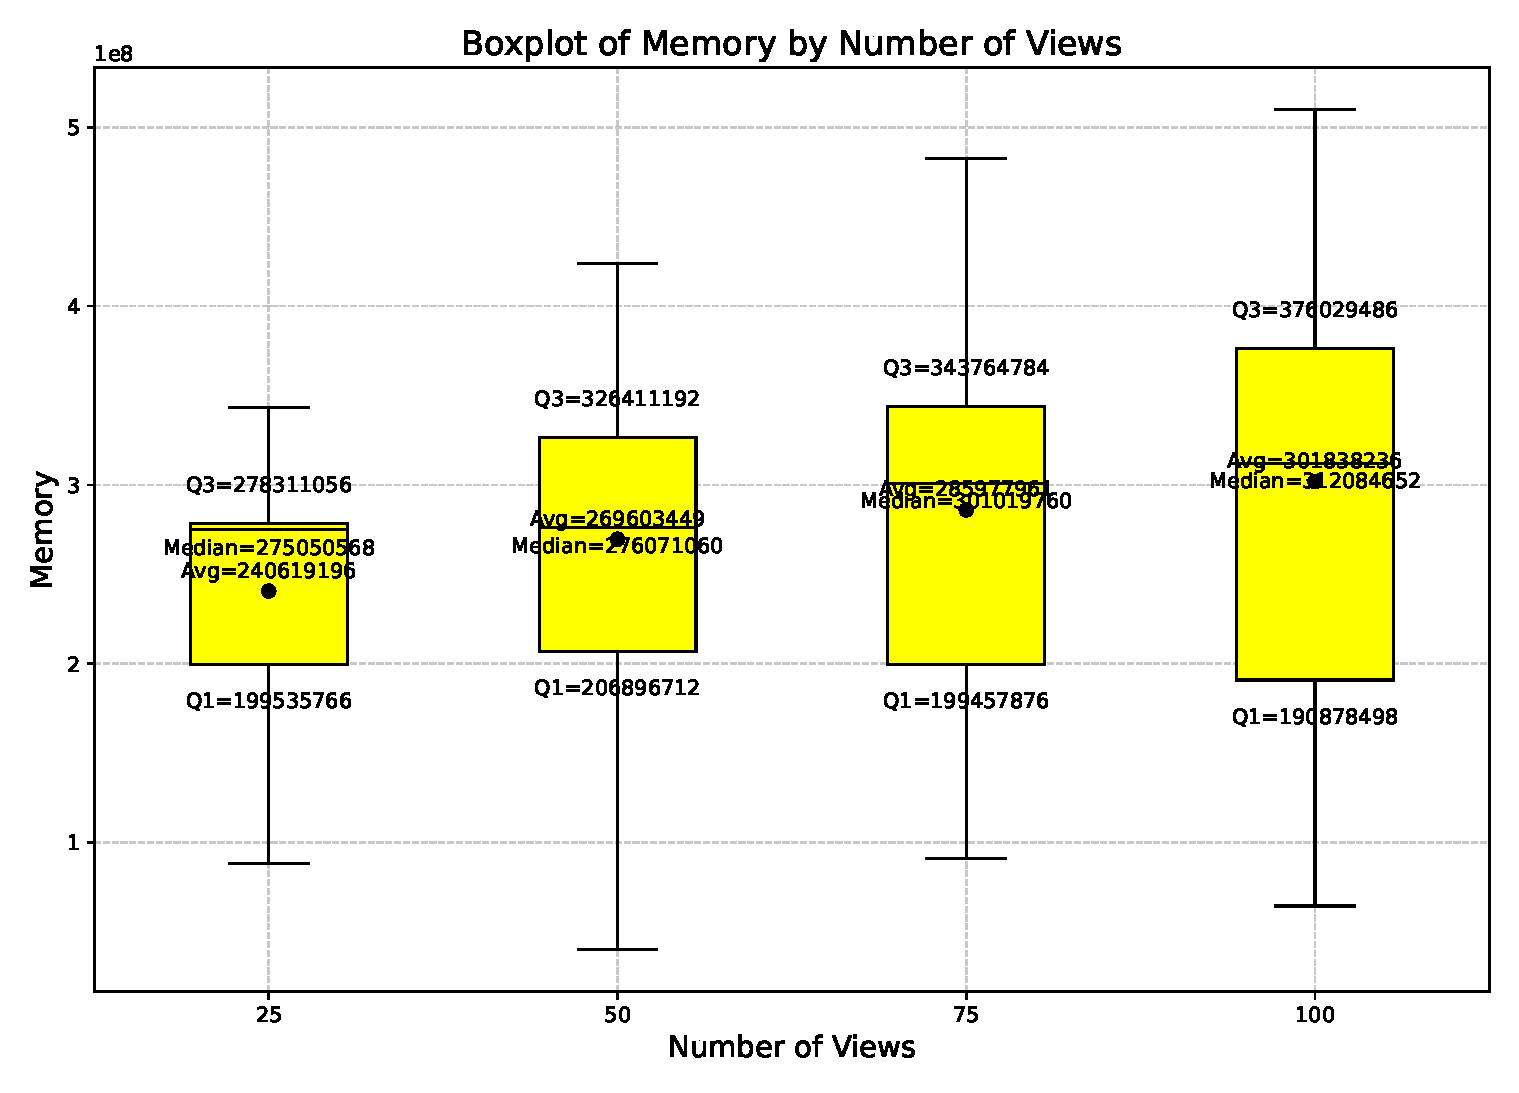
\includegraphics[width = 0.3\textwidth]{Image/mvc_plot_view_total_memory.pdf}
    \caption{Memory Used With The Number Of Views (mvc)}
    \label{fig:enter-label}
\end{figure}

\begin{figure}
    [h]
    \centering
    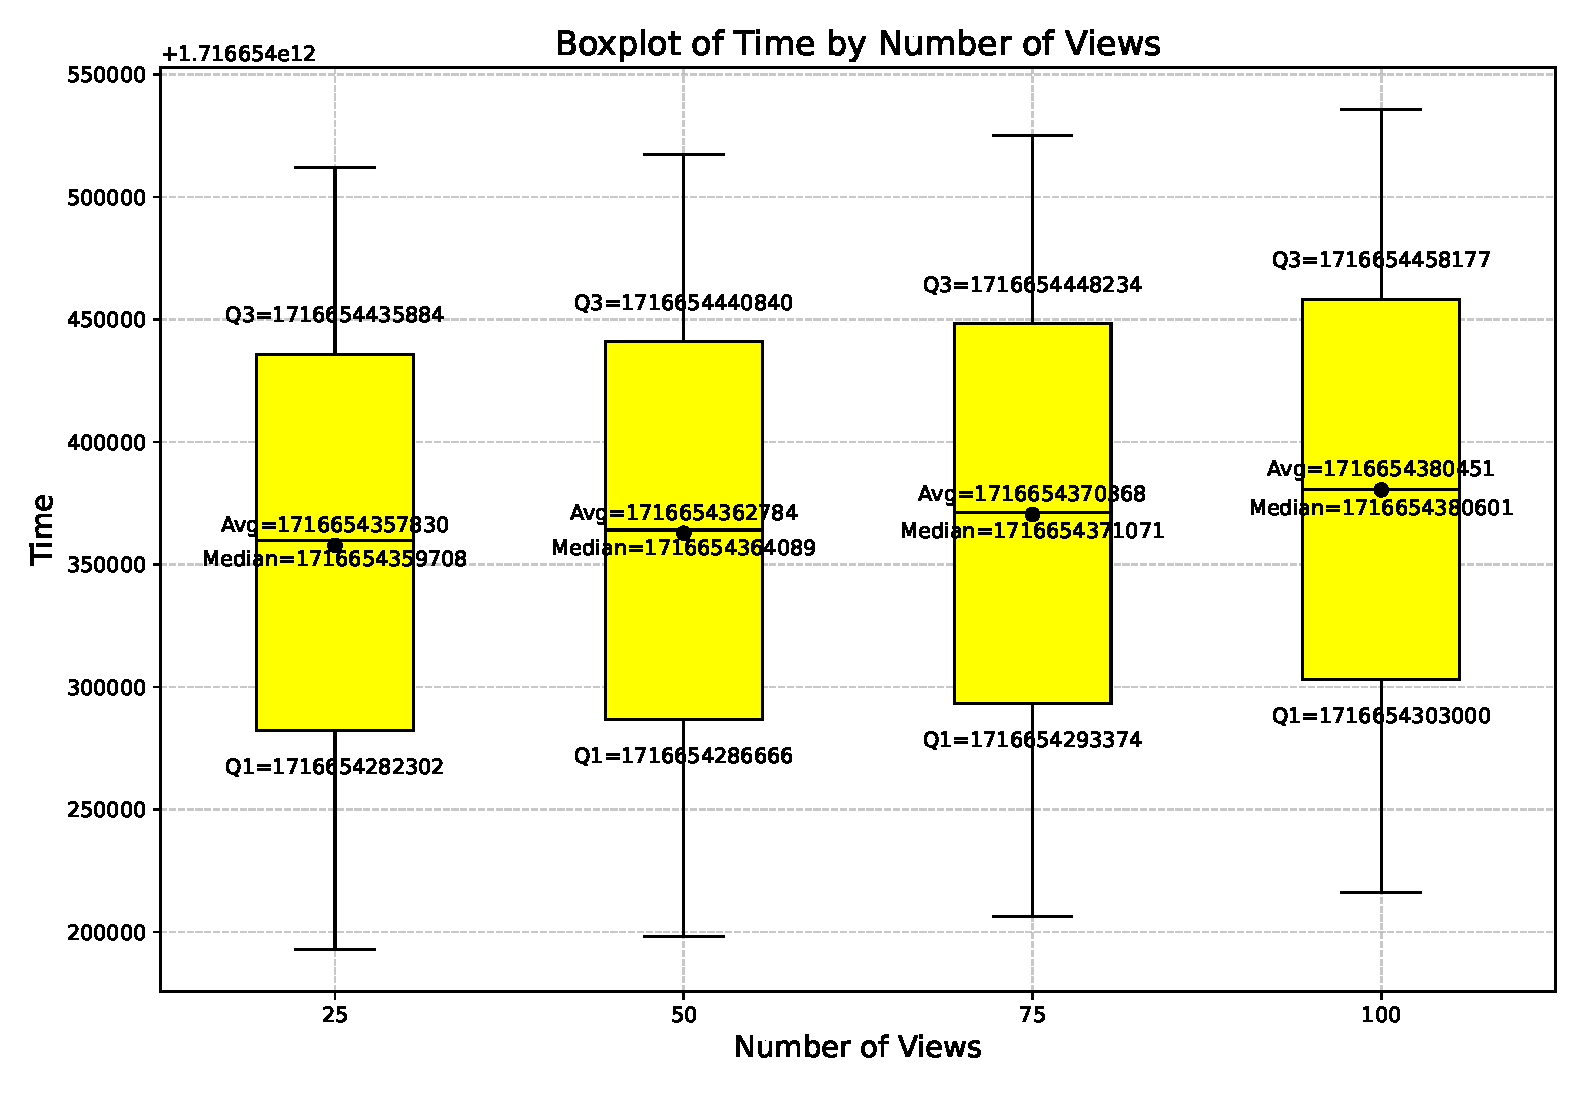
\includegraphics[width = 0.3\textwidth]{Image/mvc_plot_view_total_time.pdf}
    \caption{Times Needed With The Number Of Views (mvc)}
    \label{fig:enter-label}
\end{figure}

\subsection{MVP Test Results}

The MVP architechture managed to completed the test with 11 minutes time. with the following results produced.

\begin{figure}
    [h]
    \centering
    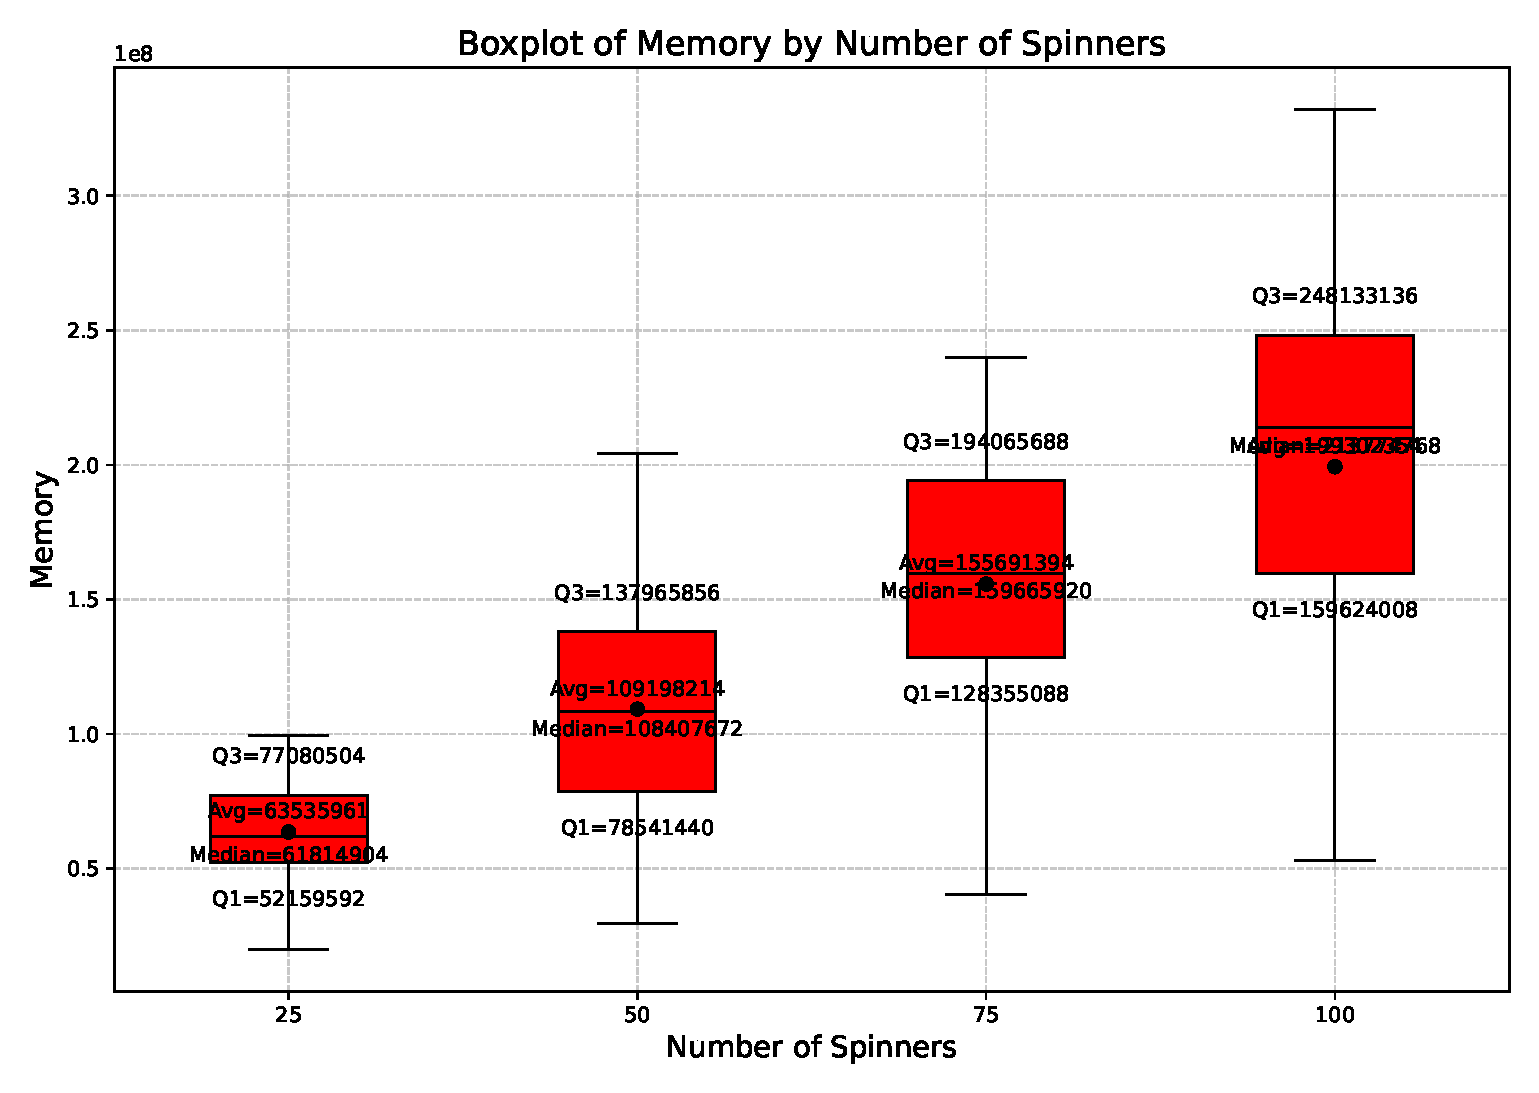
\includegraphics[width = 0.3\textwidth]{Image/mvp_plot_spin_total_memory.pdf}
    \caption{Memory Used With The Number Of Spinners Used (mvp)}
    \label{fig:enter-label}
\end{figure}

From figure 12 we can conclude that with more spinners to work with, more memories will be needed to complete the task. And the time it take to complete task can also be seen with a slight increase with more spinners, this marks the first difference between the MVC and the MVP architechture (figure 13).

\begin{figure}
    [h]
    \centering
    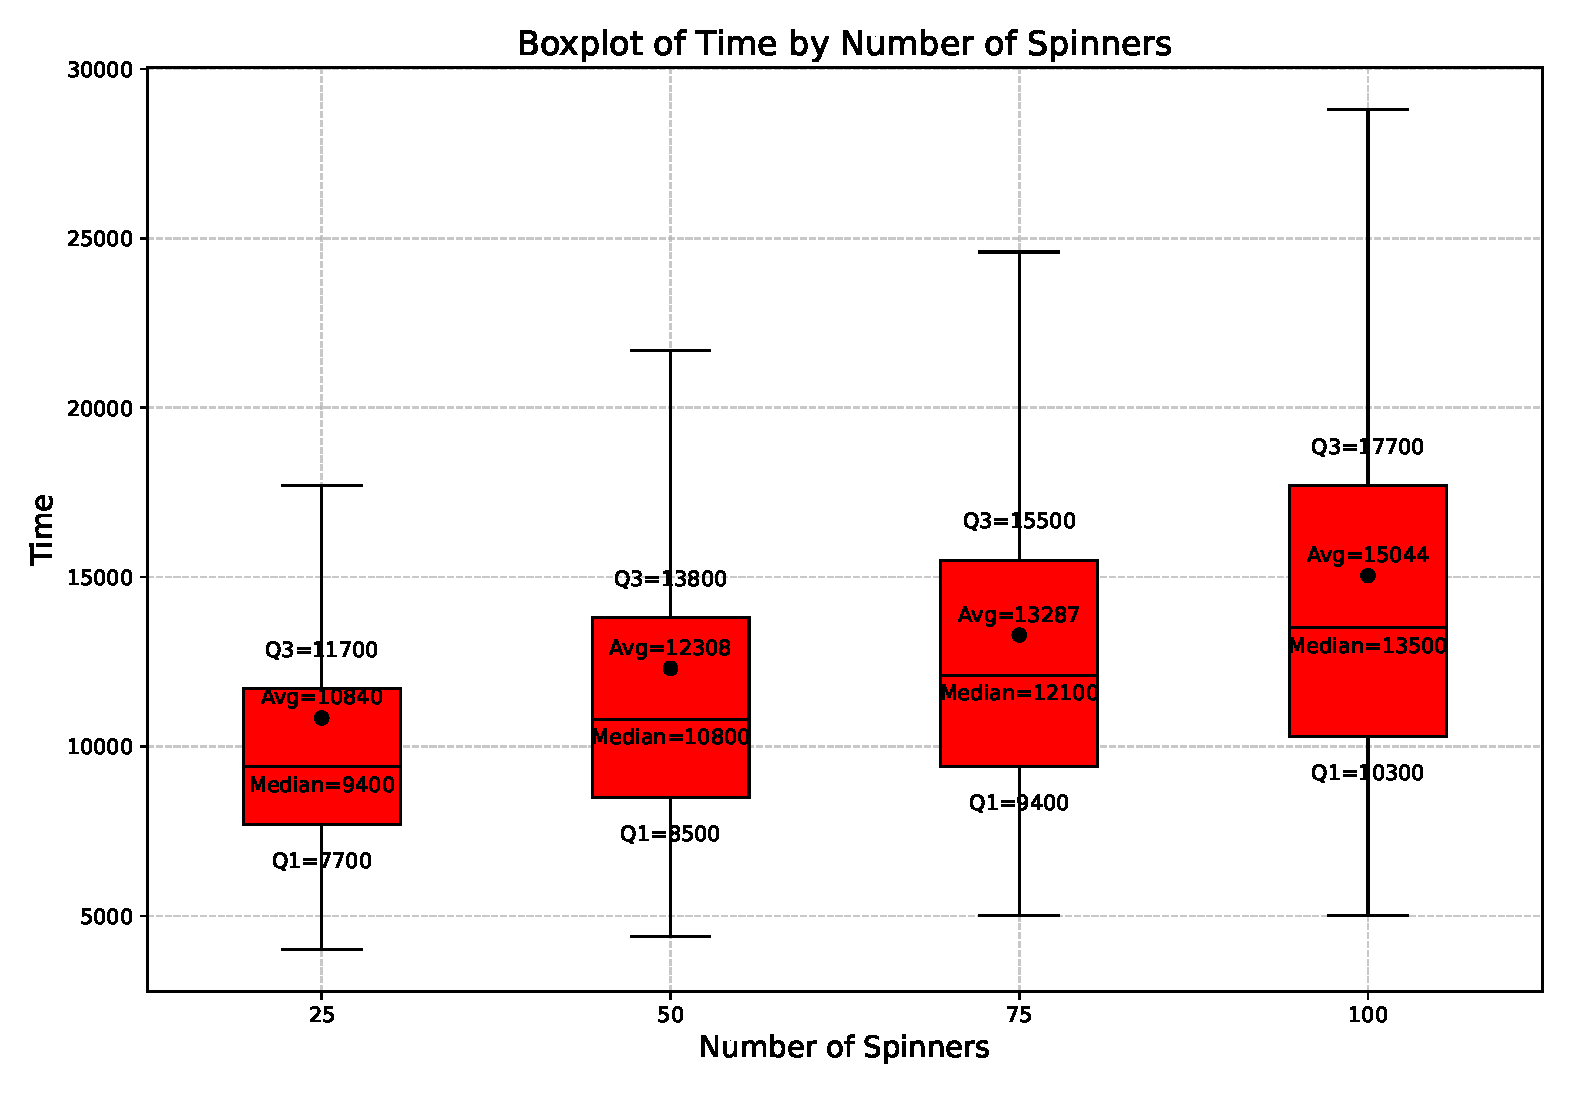
\includegraphics[width = 0.3\textwidth]{Image/mvp_plot_spin_total_time.pdf}
    \caption{Times Needed With The Number Of Spinners Used (mvp)}
    \label{fig:enter-label}
\end{figure}
\begin{figure}
    [h]
    \centering
    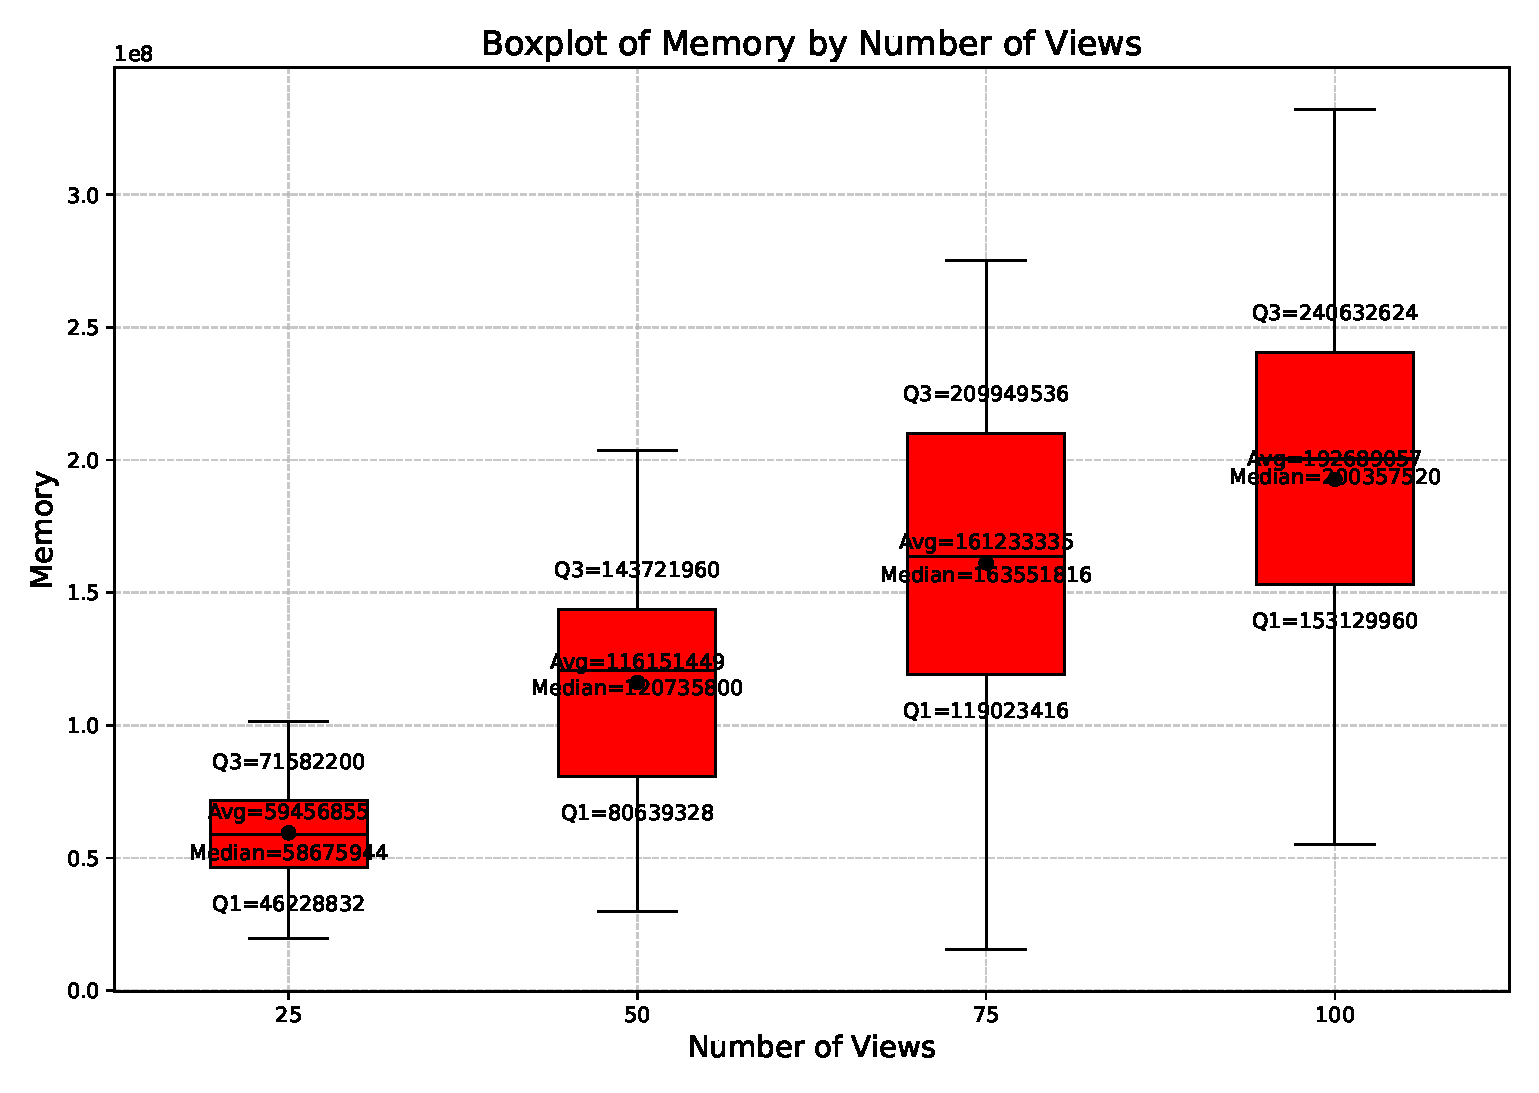
\includegraphics[width = 0.3\textwidth]{Image/mvp_plot_view_total_memory.pdf}
    \caption{Memory Used With The Number of Views (mvp)}
    \label{fig:enter-label}
\end{figure}
\begin{figure}
    [h]
    \centering
    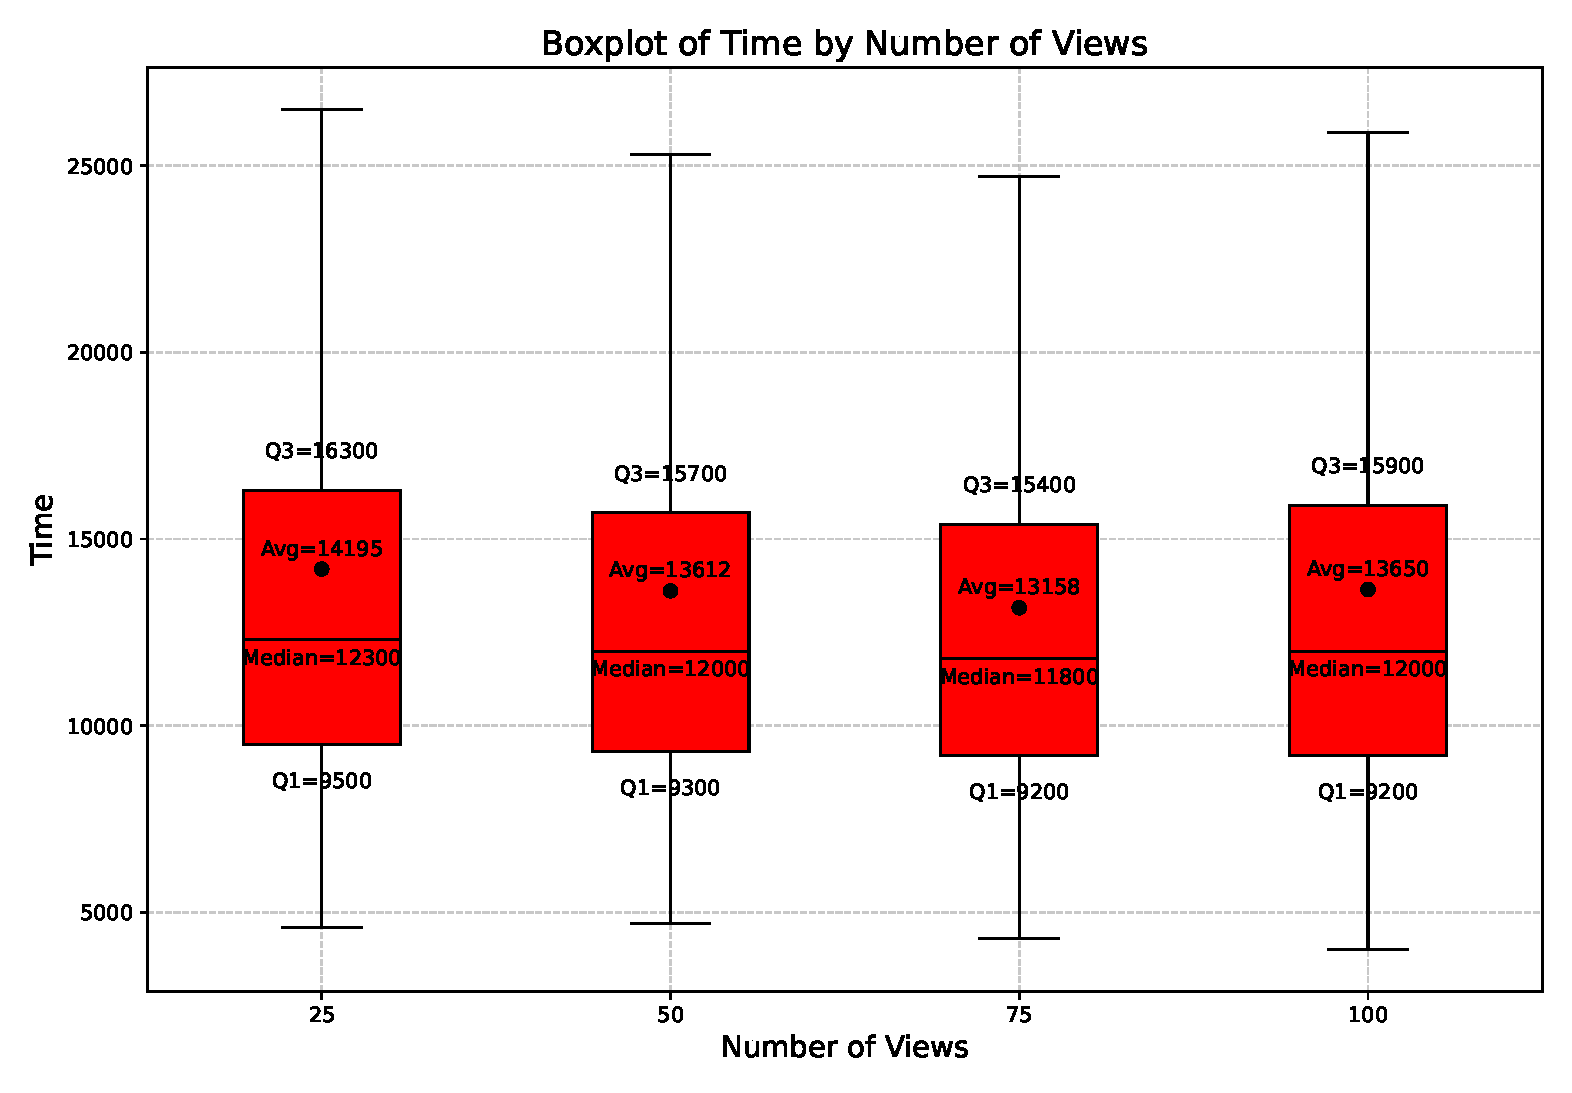
\includegraphics[width = 0.3\textwidth]{Image/mvp_plot_view_total_time.pdf}
    \caption{Times needed With The Number of Views (mvp)}
    \label{fig:enter-label}
\end{figure}
In figure 14, it also shows that the more views there is, more memories will be needed but the time it need to complete the task doesn't get affected by the number of views(figure 15).
\section{conclusion}

From the data that have been collected it seems both MVC and MVP has it's own strenght and weakness the MVC while being the faster one being able to complete the test with a mere 5.7 minutes came with a cost of more memories will be used. If both compared to each other then the boxplot can be seen as following.
\begin{figure}
    [h]
    \centering
    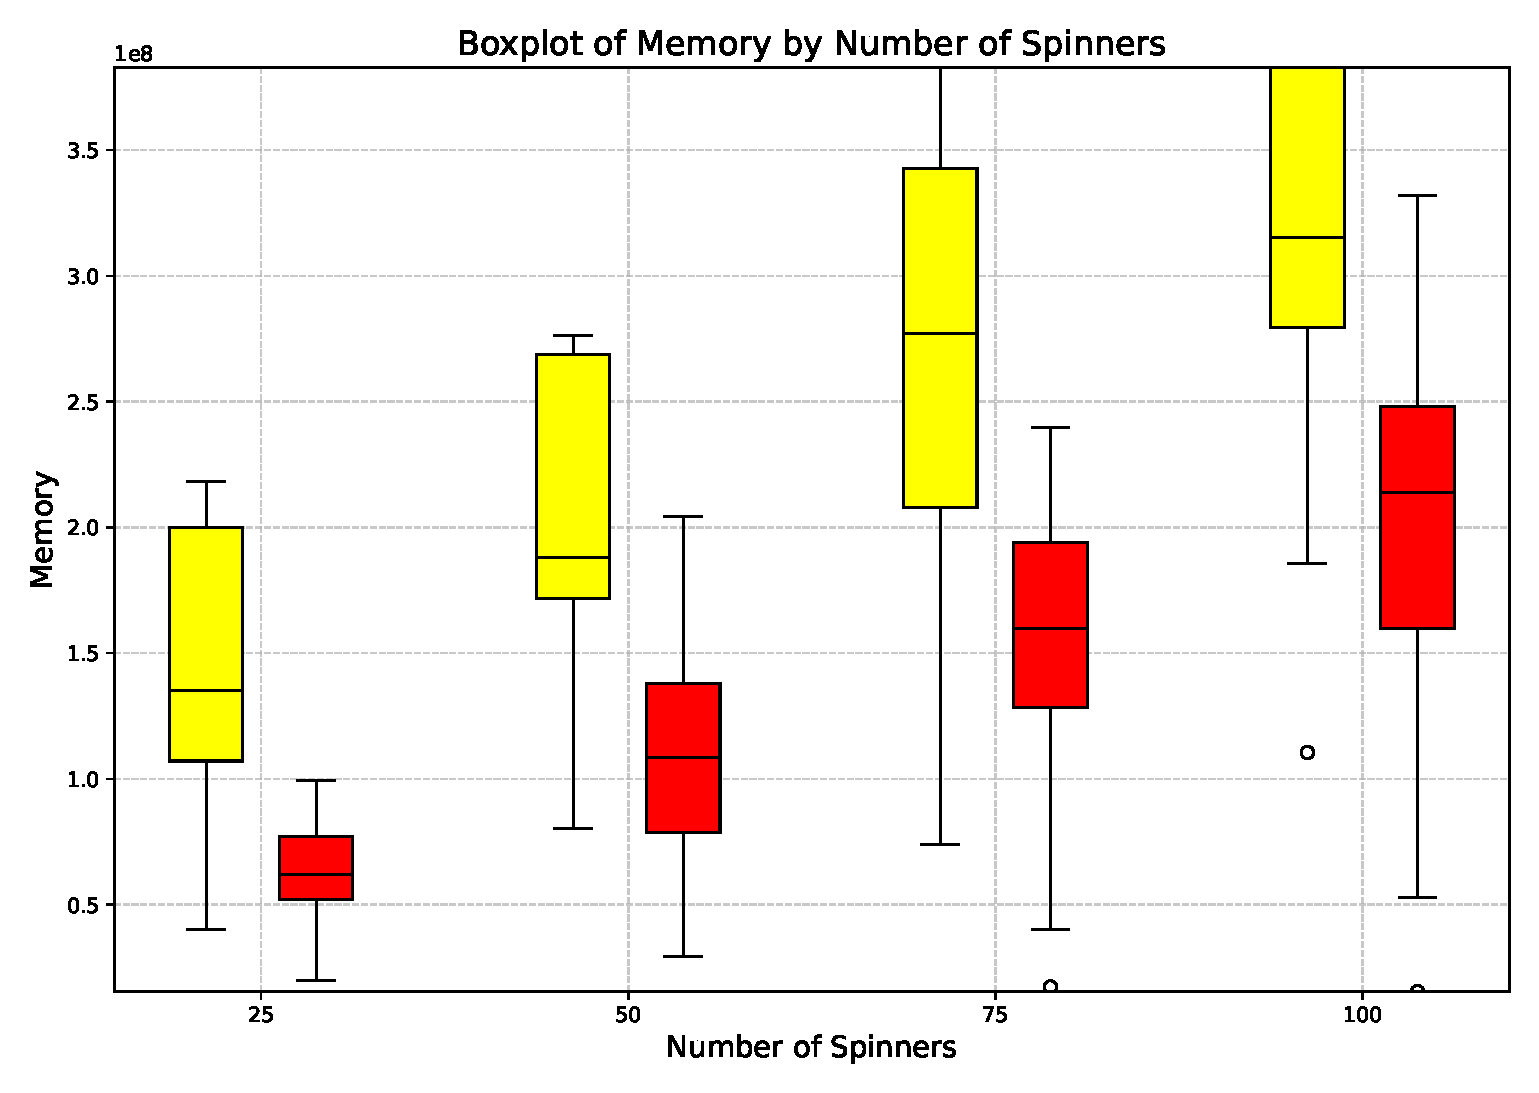
\includegraphics[width = 0.3\textwidth]{Image/mvc_vs_mvp_plot_spin_total_memory.pdf}
    \caption{Memory used With The Number of spinners (yellow mvc and red is mvp)}
    \label{fig:enter-label}
\end{figure}
\begin{figure}
    [h]
    \centering
    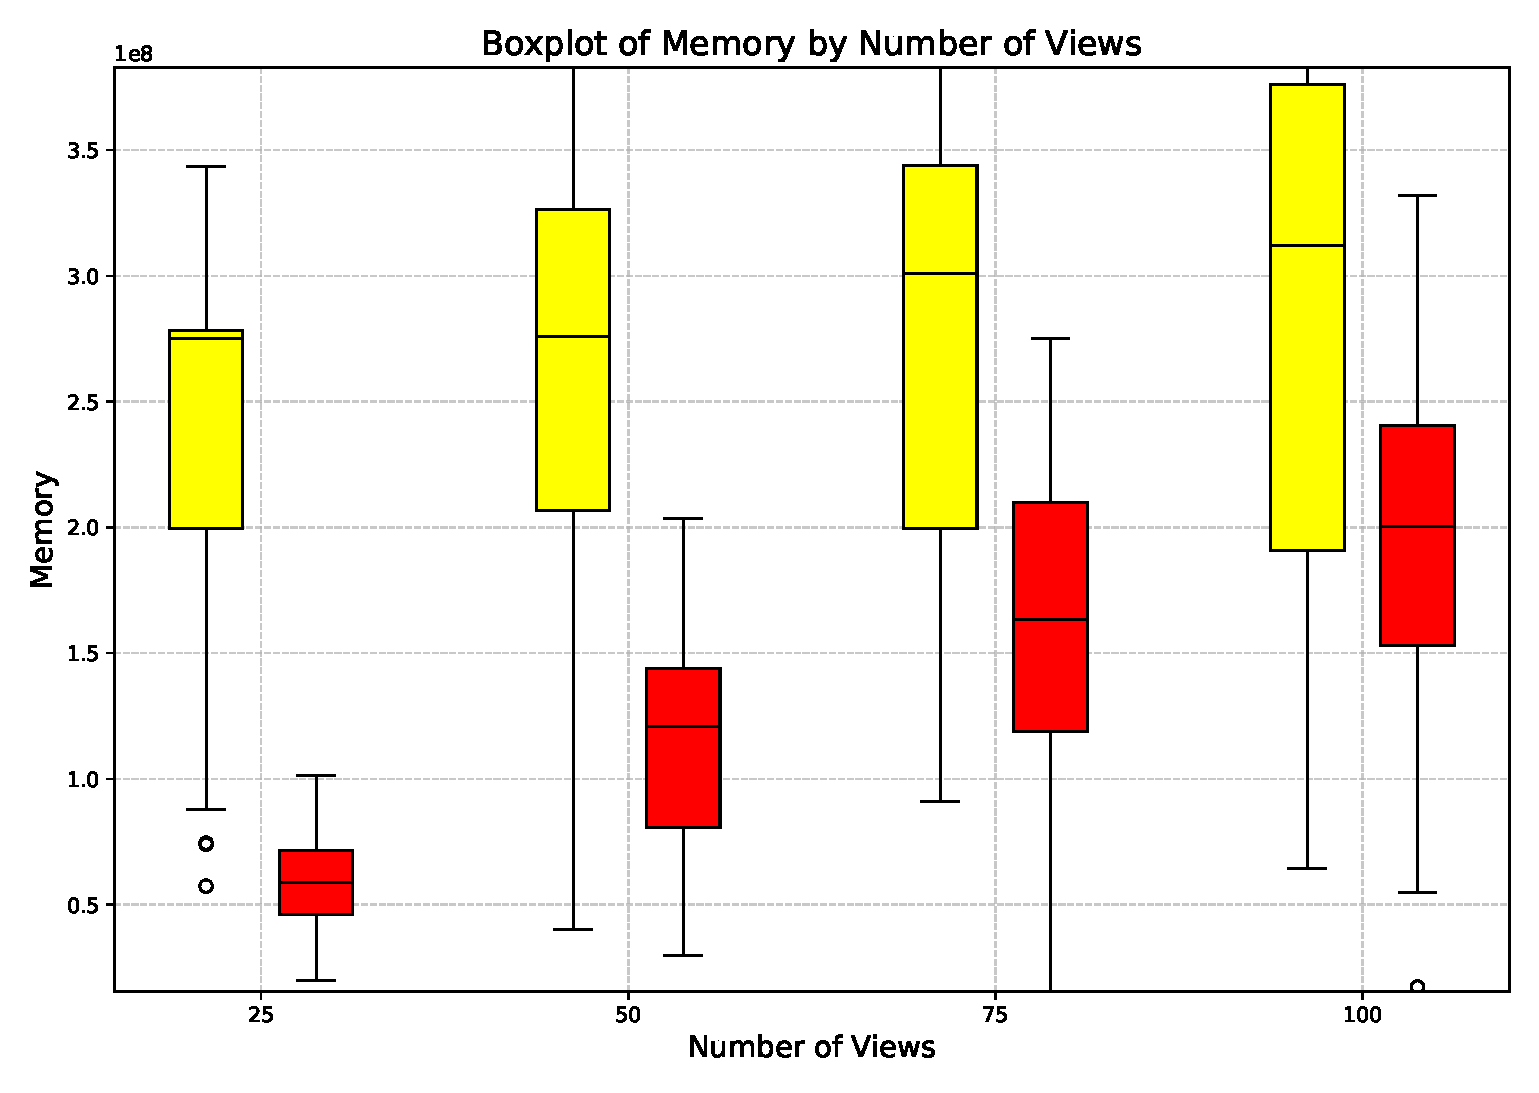
\includegraphics[width = 0.3\textwidth]{Image/mvc_vs_mvp_plot_view_total_memory.pdf}
    \caption{Memory used With The Number of views (yellow mvc and red is mvp)}
    \label{fig:enter-label}
\end{figure}
A very large difference can be seen between both architechture, although the MVP finished the test with 11 minutes, the memory used to complete the test is very low compared to the MVC architechture. With this the test is concluded and authors hope this can help to whomever that may read this.



\bibliographystyle{ieeetr}
\bibliography{reference}
\end{document}
